\documentclass[slidescentered]{beamer}
\usepackage[english]{babel}
\usepackage[utf8x]{inputenc}
\usepackage[T1]{fontenc}
\usepackage{color}

\usetheme{UniboTesi}

\title{Unibo Thesis Example}
\supervisor{Prof. Pico de Paperis}
\cosupervisor{Dr. Archimede Pitagorico}
\subtitle{There is No Largest Prime Number}
\author{Paolino Paperino}
\date{\today}
\department{Physics and Astronomy}
\school{Science}
\degree{Master Degree in Physics}

\begin{document}

	\begin{frame}[noframenumbering]
		\titlepage
	\end{frame}


	\begin{frame}{There is No Largest Prime Number}{The proof uses \textit{reductio ad absurdum}}

		\begin{theorem}
			There is no largest prime number.
		\end{theorem}

		\begin{enumerate}

  		\item<1-| alert@1> Suppose $p$ were the largest prime number.
  		\item<2-> Let $q$ be the product of the first $p$ numbers.
  		\item<3-> Then $q+1$ is not divisible by any of them.
  		\item<1-> But $q + 1$ is greater than $1$, thus divisible by some prime
  		number not in the first $p$ numbers.

		\end{enumerate}

	\end{frame}

	\begin{frame}{A title}{And a Subtitle}

		\begin{itemize}
	  	\item one
	  	\item two
		\end{itemize}

	\end{frame}

	\begin{frame}{Only an image of a Gaussian}
		\centering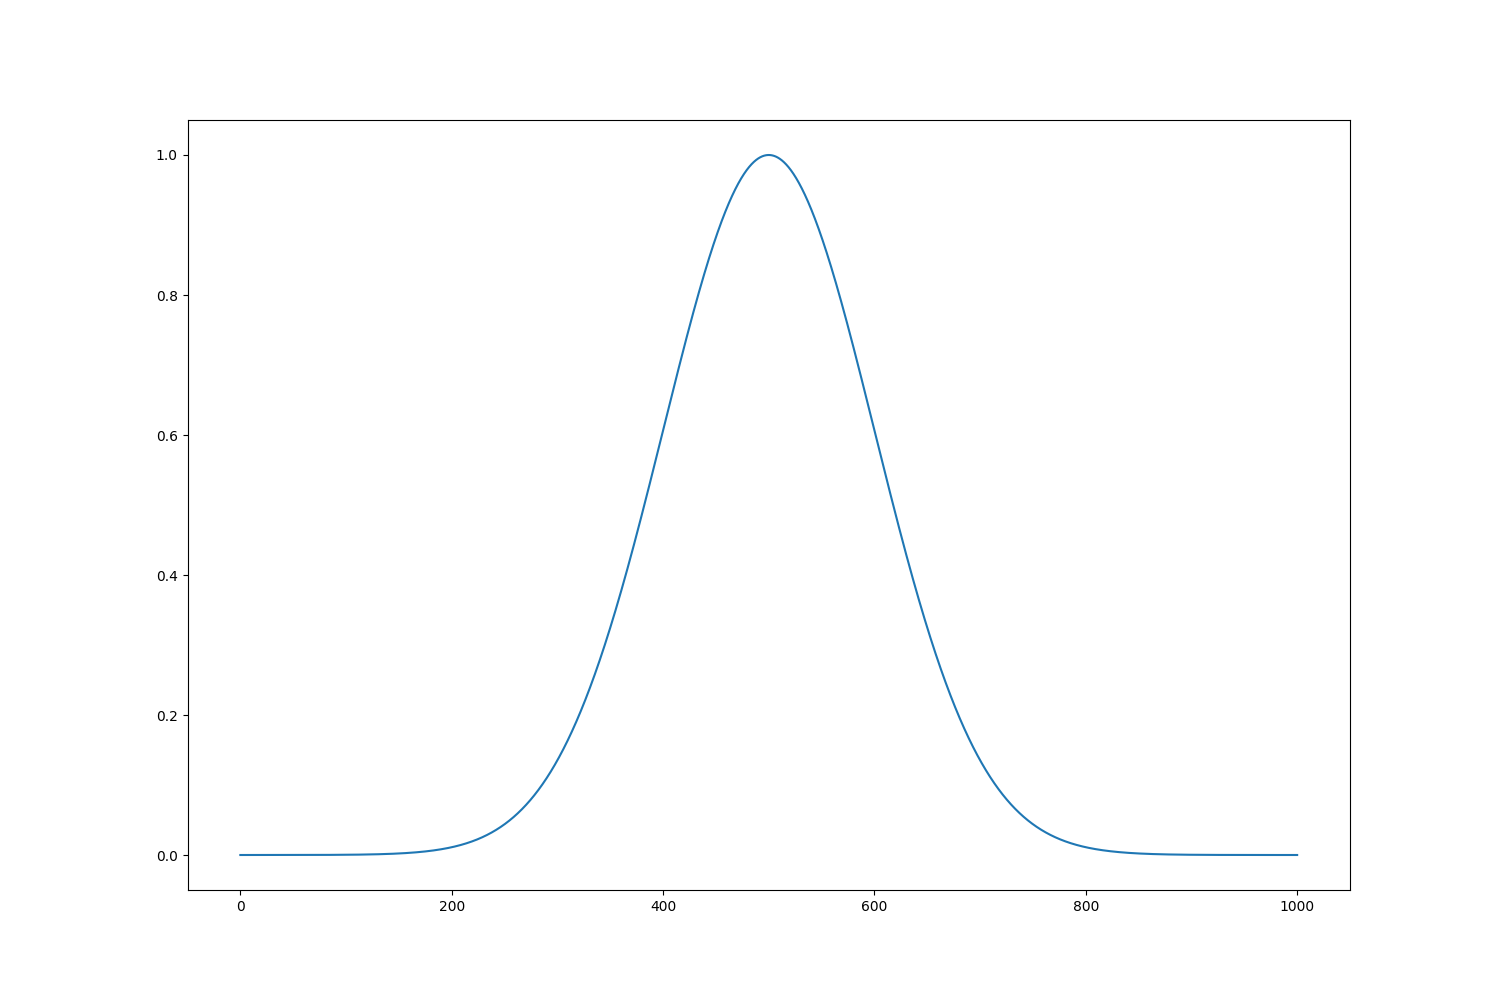
\includegraphics[width=.8\paperwidth]{./imgs/gaussian.png}
	\end{frame}

\end{document}
